\newpage
\section{Getting started}

\subsection{Your first simulation}
On both windows and linux gpvdm will install on the start menu, click on it to launch it.  Once run, a window resembling that in figure \ref{fig:new_open} will appear.  

\begin{figure}[H]
\centering
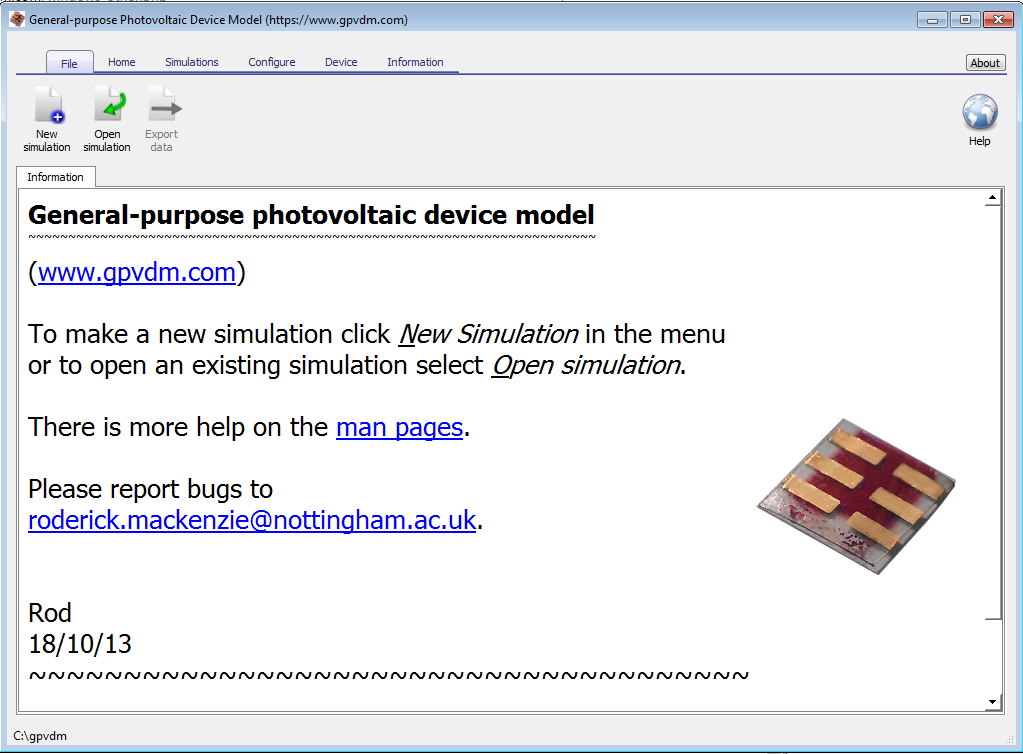
\includegraphics[width=100mm]{./images/new_open.png}
\caption{The main gpvdm simulation window.}
\label{fig:new_open}
\end{figure}

Click on the $new~simulation$ button.  This will bring up the new simulation window (see figure \ref{fig:new_new}).  From this window select the $Organic~Solar~Cell$ option and click next.  Gpvdm dumps a lot of data to disk, I therefore recommend you save the simulation to a local disk such as the C:\textbackslash drive, a network drive or usb stick drive will be far too slow for the simulation to run.  I would also not save the simulation onto OneDrive or Dropbox as they are also too slow and saving it there will generate a lot of network traffic.  If you are a power user doing a lot of fitting of experimental data I would also recommend (at your own risk(!)) disabling any extra antivirus software you have installed, as quite often the antivirus software can't keep up with the read/writes to disk.

\begin{figure}[H]
\centering
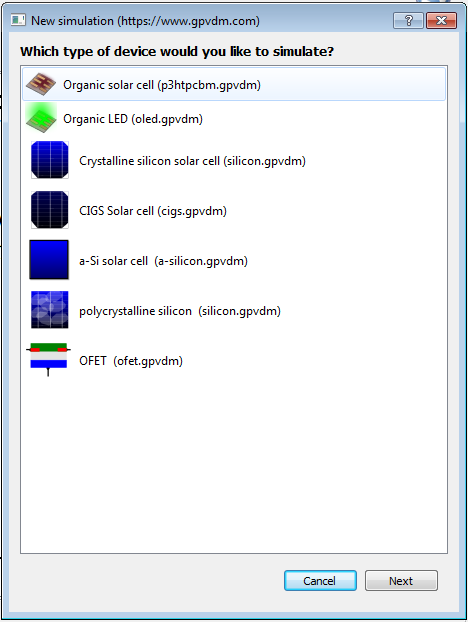
\includegraphics[width=50mm]{./images/new.png}
\caption{New simulation window}
\label{fig:new_new}
\end{figure}

Once you have saved the simulation, the main gpvdm simulation window will be brought up (see figure \ref{fig:simple_interface}). You can look around the structure of the solar cell, by dragging the picture of the solar cell with your mouse.  Try pressing on the buttons beneath the red square, they will change the orientation to the xy, yz or xz plane. Notice the x,y,z origin marker in the bottom left of the 3D window.  The icon with four squares will give you an orthographic view of the solar cell.


\begin{figure}[H]
\centering
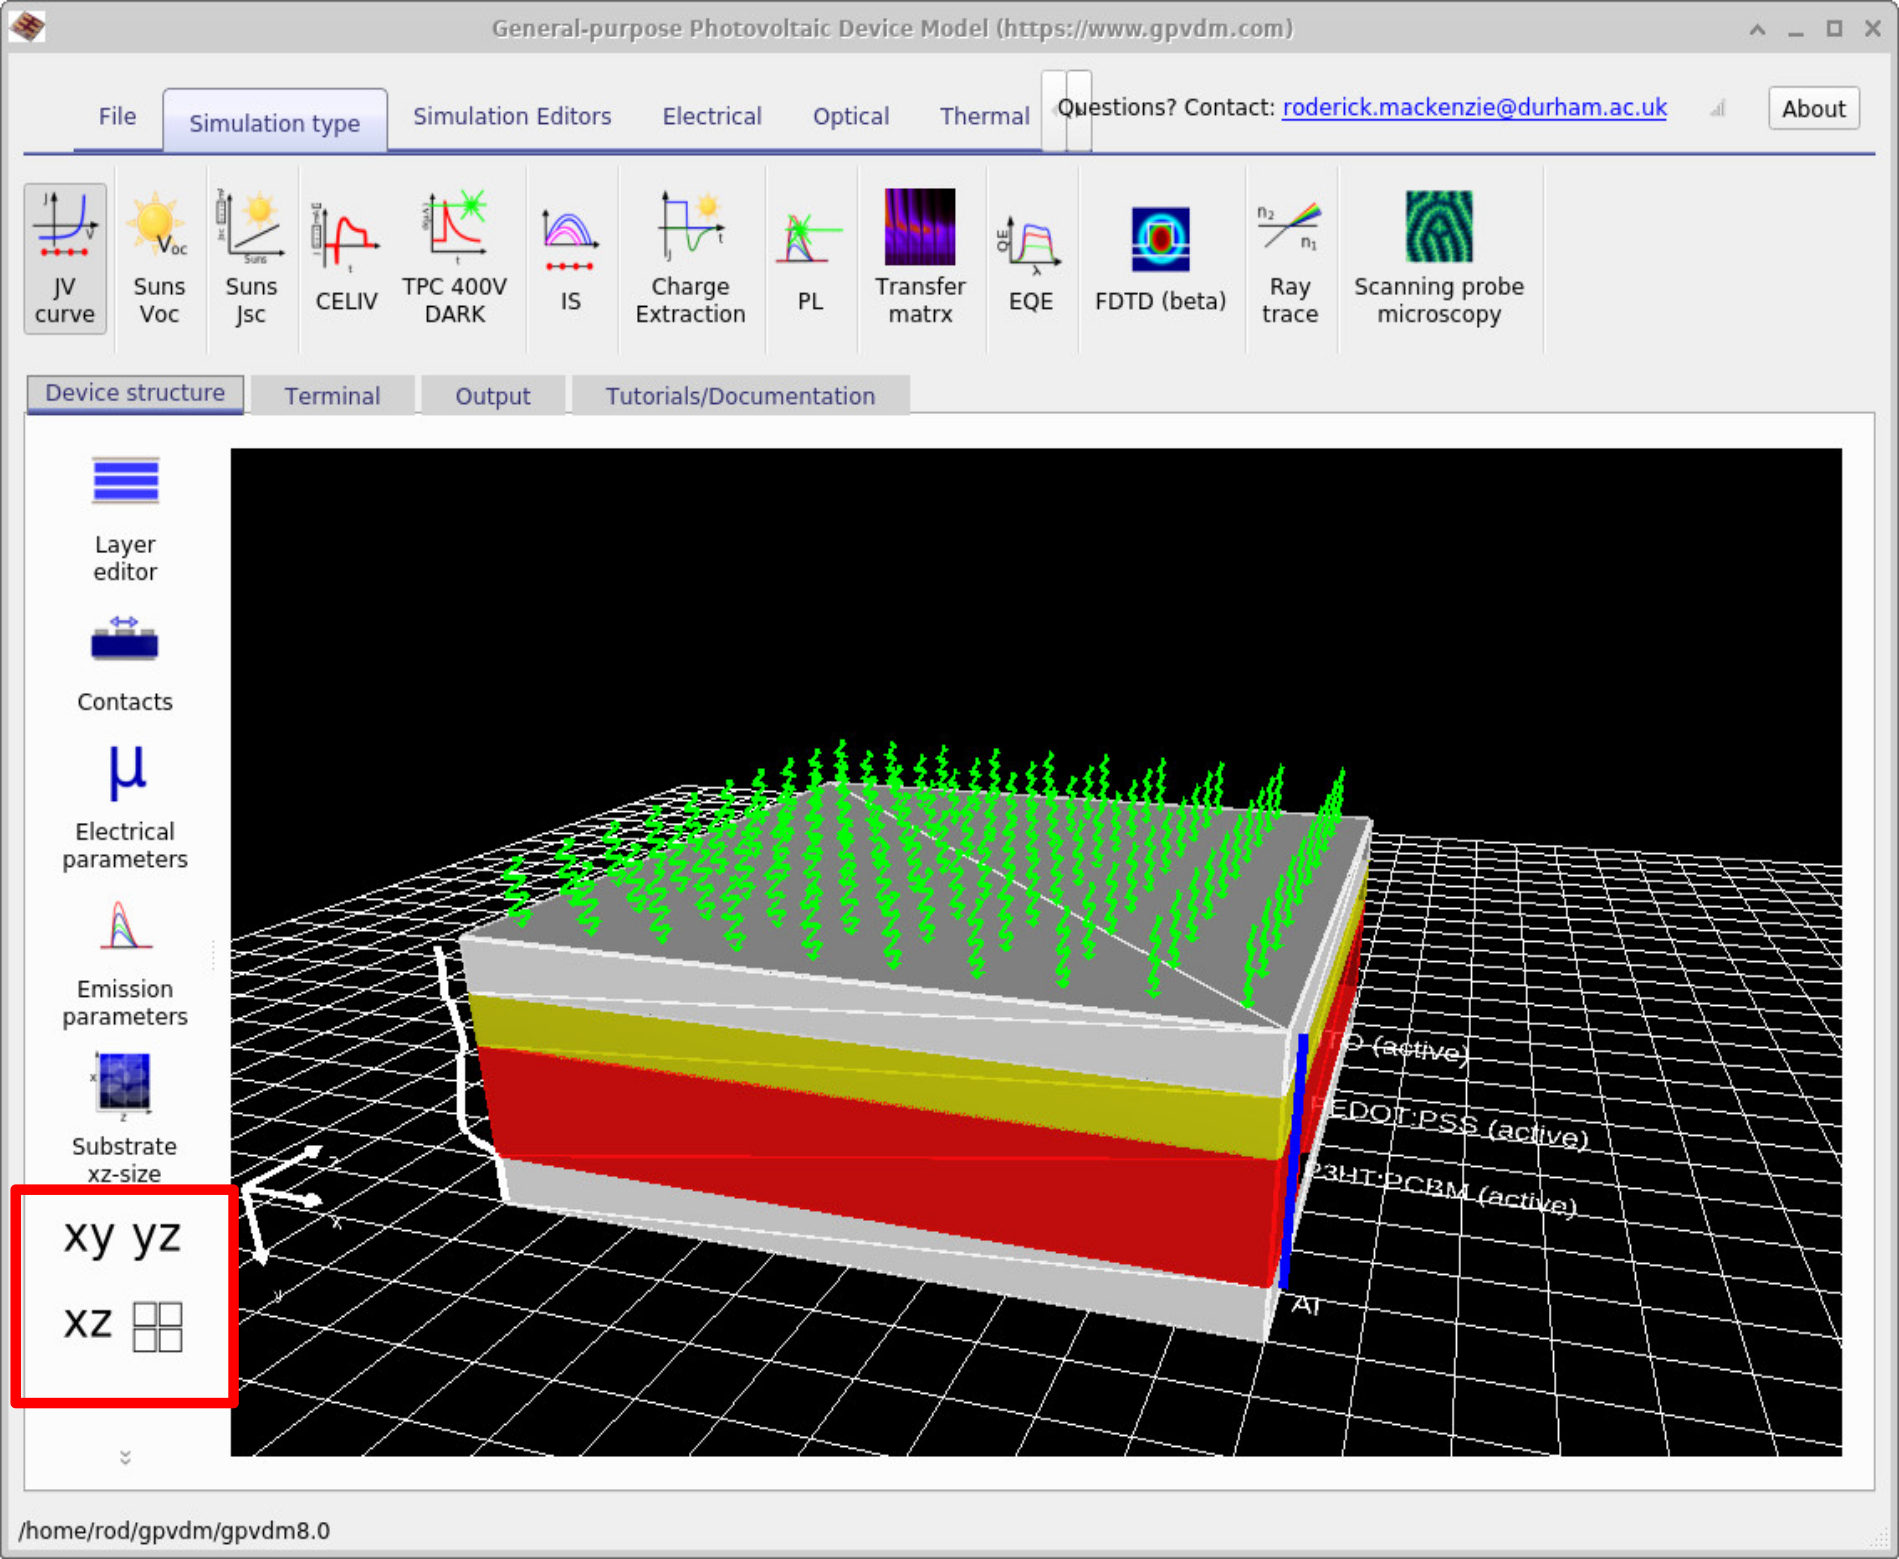
\includegraphics[width=100mm]{./images/simple_interface.png}
\caption{The main gpvdm simulation window}
\label{fig:simple_interface}
\end{figure}

Click on the button called "Run simulation" (hint it looks like a blue play button and is located in the "file" one to the right of the "Simulation type ribbon" ).  This will run the simulation.  On slower computers it could take a while. Once the simulation is done, click on the $Output$ tab (see figure \ref{fig:output}), there you will see a list of files the simulation has written to disk. Key files are listed in the table below:

\begin{table}[H]
\begin{center}
\begin{tabular}{ |c|c|c| } 
 \hline
	File name 			& 	Description  \\ 
 \hline
	$jv.dat$ 			&	Current voltage curve \\ 
	$charge.dat$ 		&	voltage charge density\\ 
	$device.dat$ 		&	The 3D device model\\ 
	$fit_data*.inp$ 	&	Experimental fit data (for demo)\\
	$k.csv$ 			&	Recombination constant k\\ 
	$reflect.dat$ 		&	Optical reflection from device\\ 
	$transmit.dat$ 		&	Optical transition through device\\ 
	$snapshots$ 		&	Electrical snapshots see \ref{sec:snapshots}\\
	$optical\_snapshots$&	Optical snapshots see \ref{sec:snapshotsoptical} \\
	$sim\_info.dat$ 	&	Calculated $V_{oc}$, $J_{sc}$ etc.. see \ref{sec:siminfo}   \\
	$cache$ 			&	Cache see \ref{sec:cache}  \\
 \hline
\end{tabular}
\caption{Files produced by the JV simulation}
\label{fig:output}
\end{center}
\end{table}

\begin{figure}[H]
\centering
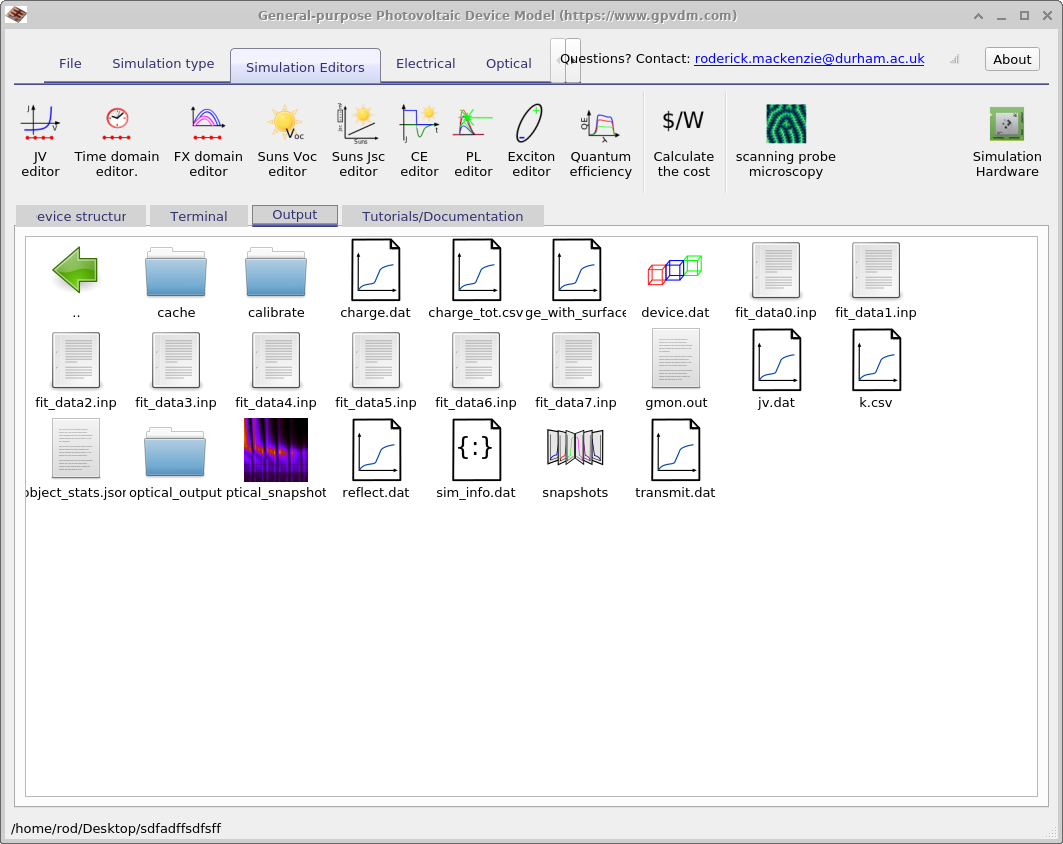
\includegraphics[width=100mm,height=70mm]{./images/output.png}
\caption{The output tab this is just like windows file explorer, you can explore the simulation directory tree.}
\label{fig:output}
\end{figure}

Try opening $jv.dat$. This is a plot of the voltage applied to the solar cell against the current generated by the device.  These curves are also sometimes called the 'charistic diode curve', we can tell a lot about the solar cell's performance by looking at these curves.  Hit the 'g' key to bring up a grid.  Place this result in your report, [Hint: you can use ctrl+c to copy the plot to the clipboard.]

\begin{figure}[H]
\centering
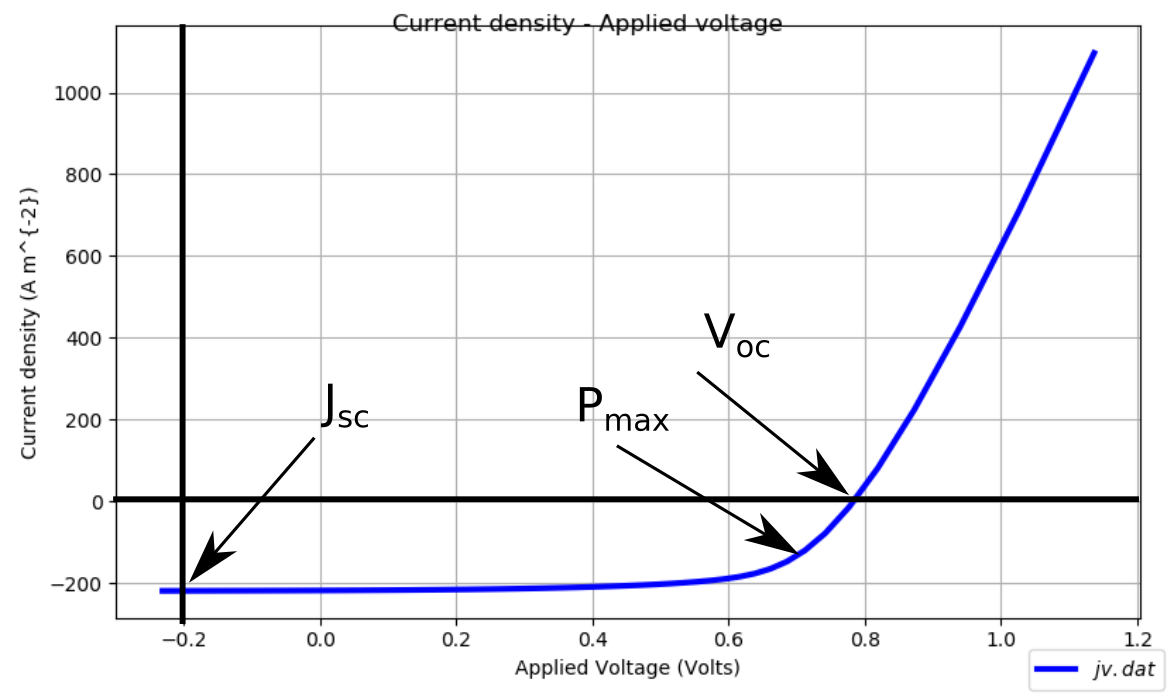
\includegraphics[width=100mm]{./images/jv_curve.png}
\caption{The output tab}
\label{fig:jv_curve}
\end{figure}


Now try opening up the file $sim\_info.dat$, this file displays information on the performance of the solar cell, such as the Open Circuit Voltage ($V_{oc}$ - the maximum Voltage the solar cell can produce when iluminated), efficiency ($\eta$ - the efficiency of the cell) , and short circuit current ($J_{sc}$ - the maximum current the cell can produce when it is illuminated).  Figure \ref{fig:jv_curve}, shows where you can find these values on the JV curve.

\subsection{Editing device layers}

\begin{figure}[H]
\centering
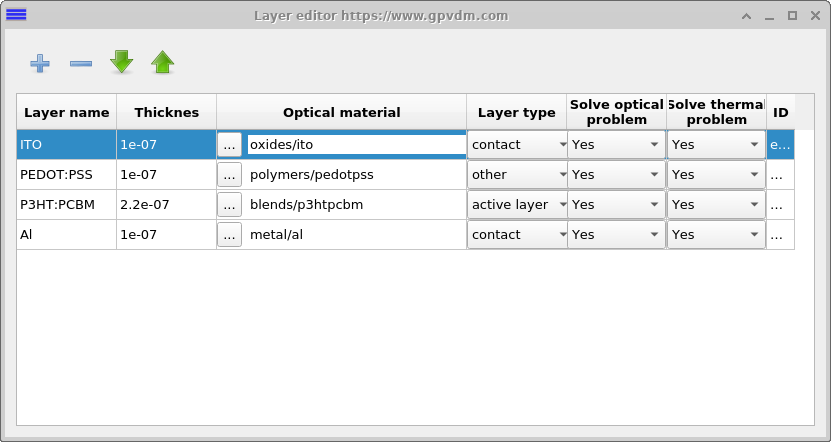
\includegraphics[width=100mm,height=70mm]{./images/layer_editor.png}
\caption{The output tab}
\label{fig:jv_curve}
\end{figure}

\subsection{Editing electrical materials}

\begin{figure}[H]
\centering
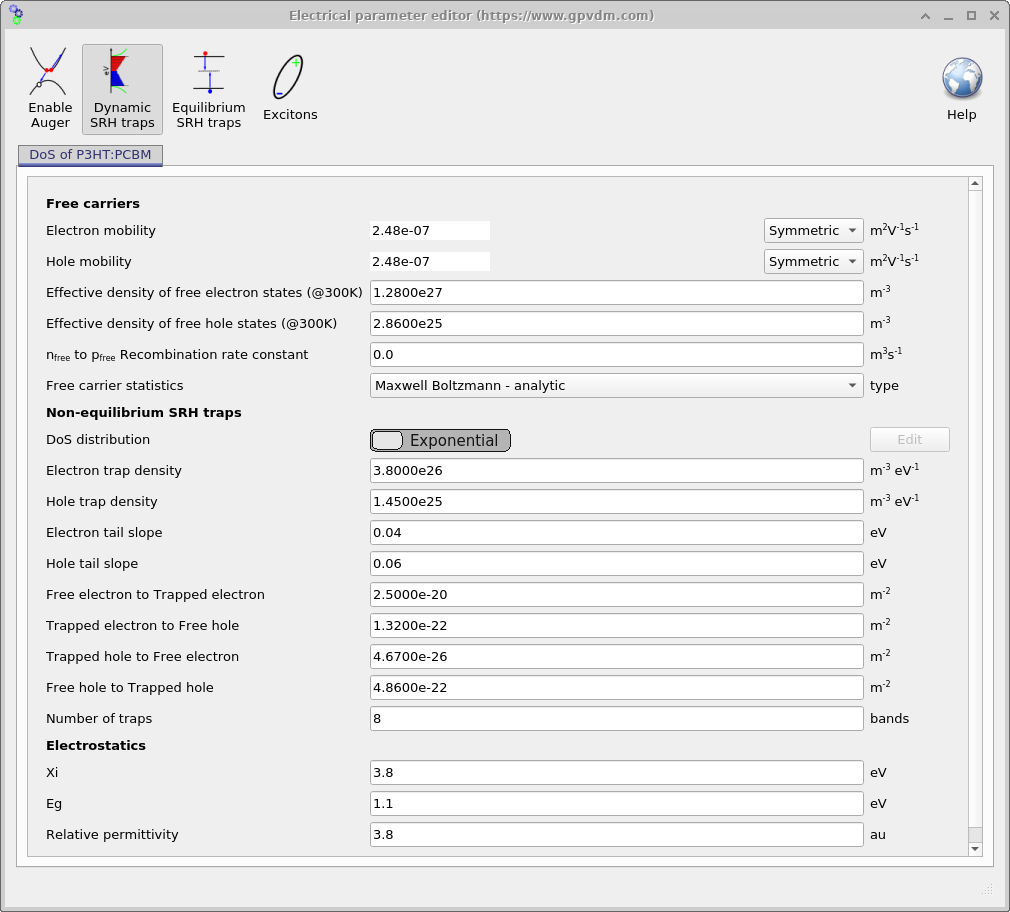
\includegraphics[width=100mm,height=70mm]{./images/dos_editor.png}
\caption{The output tab}
\label{fig:jv_curve}
\end{figure}
